% -*-latex-*-
%\documentclass[handout]{beamer}
\documentclass[12pt]{beamer}
\usepackage{etex}

\let\latexput\put
\usepackage{pictex}
\let\pictexput\put
\let\put\latexput

\usepackage{graphicx,mathdots}
\setbeamertemplate{footline}[frame number]
\setbeamercovered{transparent}
\title{Inbreeding}
\author{Alan R. Rogers}
\date{\today}
%\UseRawInputEncoding
\begin{document}

\frame{\titlepage}

%\frame{Read: Joshi:N-10.1038-nature14618}

\begin{frame}
\frametitle{Inbreeding depression in corn}
\begin{columns}
\column{0.6\textwidth}
 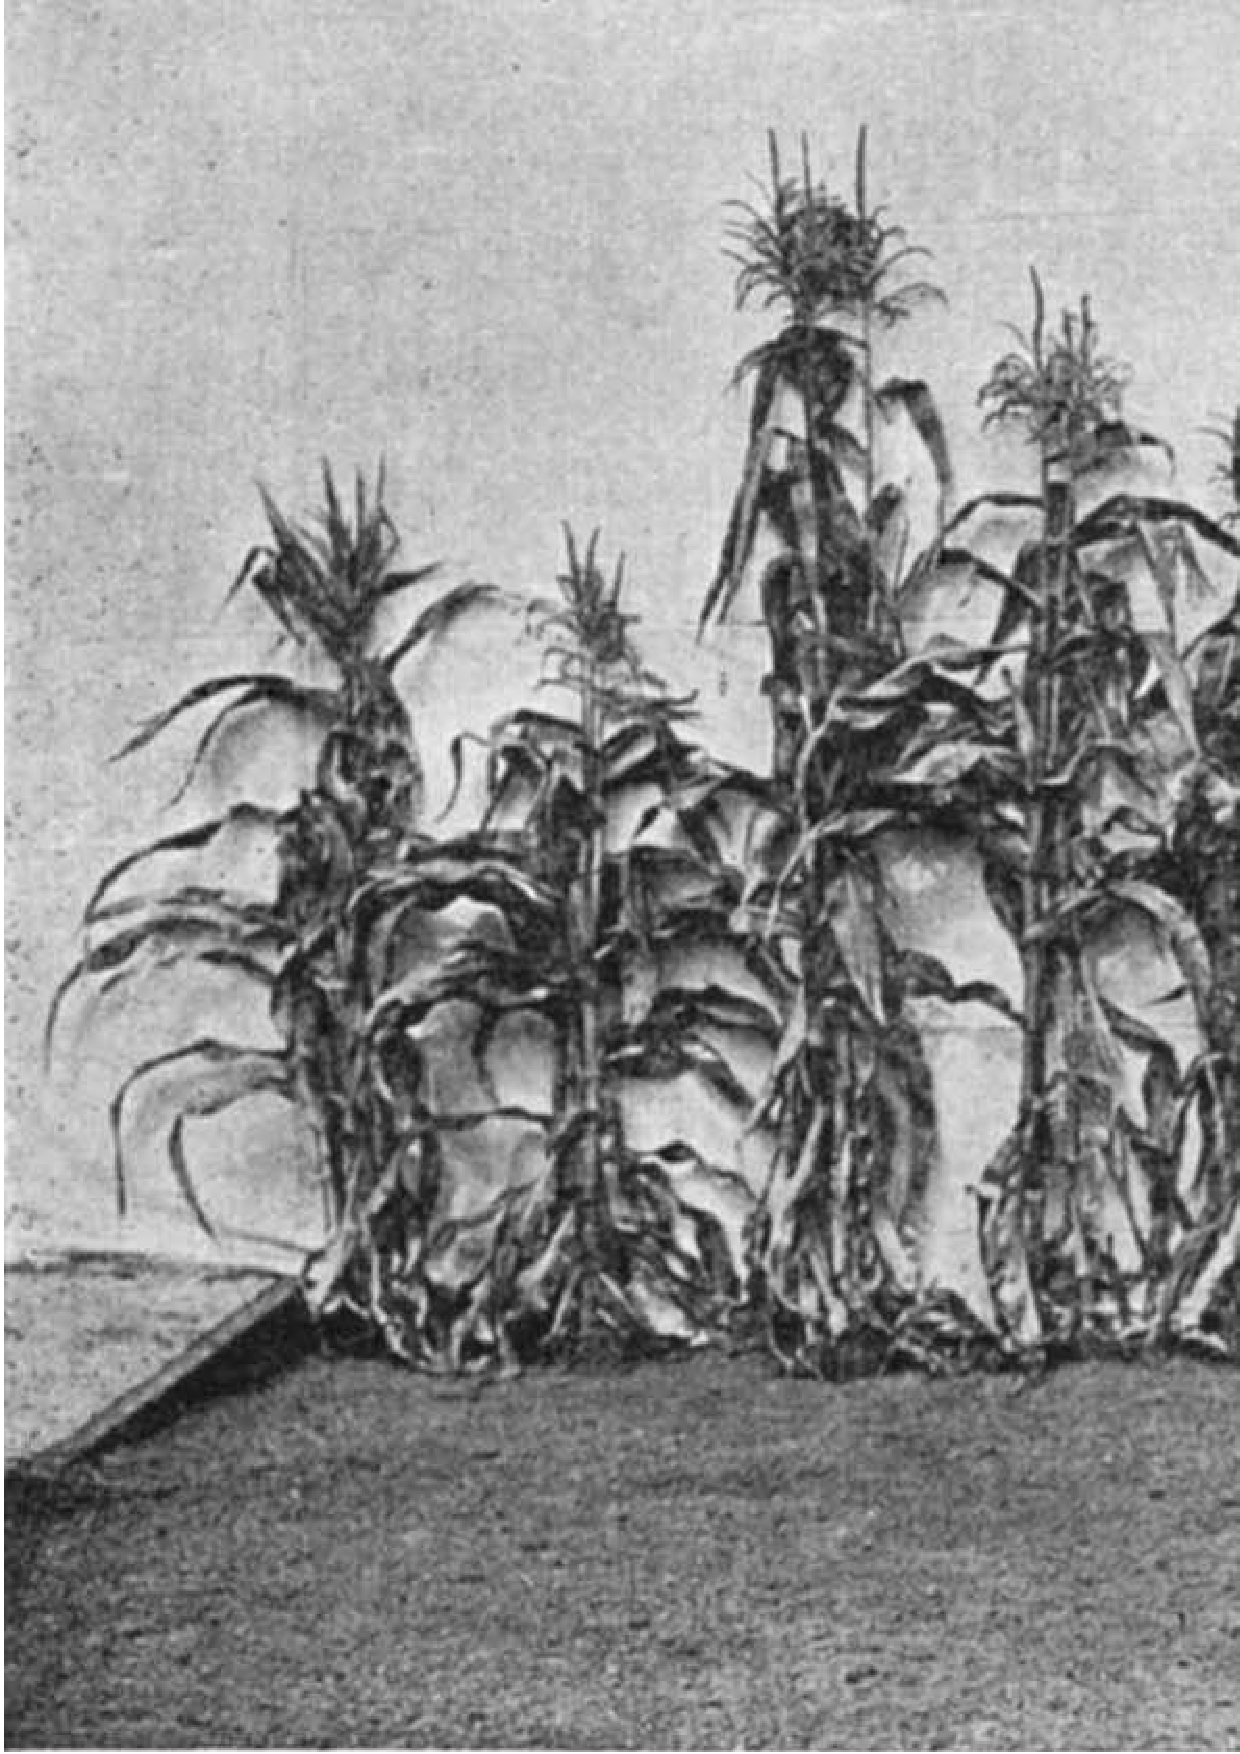
\includegraphics[width=\textwidth]{corn.png}\\
\mbox{}\hfill\textsc{\footnotesize (Jones 1924)}
\column{0.4\textwidth}\raggedright
\begin{itemize}
\item Two plants on left are from inbred homozygous strains.
\item Next: the $F_1$ offspring of these strains
\pause
\item Then offspring $(F_2)$ of two $F_1$s.
\item Then $F_3$
\item And so on.
\end{itemize}
\end{columns}
\end{frame}

\begin{frame}
\frametitle{Inbreeding depression in humans}
\begin{columns}
\column{0.6\textwidth}
 \includegraphics[width=1.1\textwidth]{inbredmort.pdf}
\column{0.4\textwidth}\raggedright
Offspring of cousin marriages are less likely to survive.\\
\textsc{\footnotesize (Bittles and Neel 1994)}
\end{columns}
\end{frame}

\begin{frame}
\frametitle{Genotype frequencies without random mating}
\begin{columns}
\column{0.5\textwidth}
\[
\begin{array}{ll}
\hbox{Genotype} & \hbox{Frequency}\\
\hline
A_1 A_1 & p^2 + pqF\\
A_1 A_2 & 2pq(1-F)\\
A_2 A_2 & q^2 + pqF\\
\end{array}
\]
\column{0.5\textwidth}
Describes any bi-allelic locus.

\medskip

$F=0$ under random mating.\\
Reduces to Hardy-Weinberg.

\medskip
$F>0$ under inbreeding.
Gives excess of homozygotes.\\

\medskip
$F$ is the \emph{coefficient of inbreeding}.
\end{columns}
\end{frame}

\begin{frame}
\frametitle{Example}
\begin{columns}
\column{0.5\textwidth}
Assume $p=1/2$
\begin{tabular}{lcc}
      & \multicolumn{2}{c}{\hbox{Frequency}}\\
\hbox{Genotype} & $F=0$ & $F=0.1$\\
\hline
$A_1A_1$ & 0.25 & 0.275\\
$A_1A_2$ & 0.50 & 0.450\\
$A_2A_2$ & 0.25 & 0.275\\
\end{tabular}
\column{0.5\textwidth}
\raggedright
Inbred population has more homozygotes.\\

\bigskip

Suffers if either
\begin{itemize}
\item Heterozygotes tend to have high fitness
\item Deleterious alleles tend to be recessive.
\end{itemize}
\end{columns}
\end{frame}

\begin{frame}
\frametitle{Outline of theory}
Inbreeding increases $F$,
\pause
which increases homozygosity,
\pause
which decreases fitness.
\end{frame}

\begin{frame}
\frametitle{Decay of heterozygosity under selfing}
\large
\[
\begin{array}{rccccccccc}
\hbox{Gen.}& A_1A_1 &&&& A_1A_2 &&&& A_2A_2\\
0          &     &&&& N\\
           &     &&&\iddots& \vdots &\ddots\\[-1ex]
           &     &&\frac{1}{4}&& \frac{1}{2}&&\frac{1}{4}\\[-1ex]
           &     &\iddots&&& \vdots &&&\ddots\\
1          & \frac{1}{4}N &&&& \frac{1}{2}N   &&&&  \frac{1}{4}N\\
           &\vdots&&&\iddots& \vdots &\ddots&&&\vdots\\[-1ex]
           &  1  &&\frac{1}{4}&& \frac{1}{2}&&\frac{1}{4}&&1\\[-1ex]
           &\vdots&\iddots&&& \vdots &&&\ddots&\vdots\\
2          & \frac{3}{8}N &&&& \frac{1}{4}N   &&&&  \frac{3}{8}N   \\
\end{array}
\]
\end{frame}

\begin{frame}
\frametitle{Decay of heterozygosity under selfing}
Half of heterozygosity is lost each generation.
\end{frame}

\begin{frame}
\frametitle{What about cousin mating, or mating between sibs?}

It is \emph{extremely} difficult to work this out, using the method we
just used.

\bigskip

Between 1903 and 1915, no one could get it right.

\bigskip
\pause

Pearl (1913): Only for brother-sister matings does inbreeding reduce
heterozygosity.  [\textcolor{red}{Wrong!}]

\bigskip
\pause

Solution: build theory looking backwards in time, not forwards.
\end{frame}

\begin{frame}
\frametitle{Kinds of gene identity}
There are two senses in which a pair of gene copies may be
``identical:''
\begin{tabbing}
identity by descentxx\=:xx\=copies of same gene copy in an ancestor\kill
identity in state\>:\>copies of same allele\\
identity by descent\>:\>copies of same gene copy in an ancestor
\end{tabbing}

\medskip
Abbreviation: IBD = Identity by Descent
\end{frame}

\begin{frame}
\frametitle{Gametes $a$ and $b$ are identical by descent}
{\centering\input{figibd}\\}
\end{frame}

\begin{frame}
\frametitle{Identical in state, not by descent}
\begin{columns}
\column{0.7\textwidth}
\input{figiis}
\column{0.3\textwidth}
\raggedleft
May be IBD relative to an earlier generation.

\medskip
Not IBD relative to the pedigree shown here.

\medskip
IBD is always relative to a particular generation.
\end{columns}
\end{frame}

\begin{frame}
\frametitle{Identical neither in state nor by descent}
\centering
% Darwin-Wedgewood Genealogy
\let\put\pictexput
\mbox{\beginpicture
\setcoordinatesystem units <1cm,1cm>
\setplotarea x from -3 to 3, y from -4 to 1
%\setdots
%\axis invisible bottom ticks andacross numbered from -3 to 3 by 1 /
%\axis invisible left ticks andacross numbered from -4 to 1 by 1 /
%\setsolid
\Large
\put {$\circ$~$\bullet$} at 0 0
\circulararc 360 degrees from 0 -0.75 center at 0 0
%
\put {$\bullet$~$\circ$} at -2 -2
\circulararc 360 degrees from -2 -2.75 center at -2 -2
%
\put {$\circ$~$\bullet$} at 2 -2
\circulararc 360 degrees from 2 -2.75 center at 2 -2
%
\arrow <10pt> [.2,.67] from -0.2 0 to -1.7 -1.9
\arrow <10pt> [.2,.67] from 0.2 0 to 2.1 -1.9
%
\put {\textsf{a}} [t] at -2 -4
\put {\textsf{b}} [t] at 2 -4
\setdots
\setplotsymbol ({\small$\cdot$})
\setquadratic
\plot -1.7 -2.1  -1.5 -3  -2 -4 /
\plot  2.3 -2.1   2.5 -3   2 -4 /
\endpicture}
\let\put\latexput

\end{frame}

\begin{frame}
\frametitle{Uniting gametes}
Consider the two gametes that unite to form an individual.
\begin{itemize}
\item $F$, is the probability that they are IBD
\item What is the probability that they both carry $A_1$?
\end{itemize}
\medskip
\pause
\begin{tabular}{lc}
Event & Probability\\
\hline
IBD from $A_1$-bearing ancestor & $Fp$\\
\pause
\parbox{3in}{Descend from two random ancestors who both carry $A_1$}
  & $(1-F)p^2$\\
\hline
\end{tabular}
\pause

\medskip
\begin{eqnarray*}
P_{11} &=& Fp + (1-F)p^2\\
       &=& p^2 + pqF
\end{eqnarray*}
\end{frame}

\begin{frame}
\frametitle{All three genotypes}
\begin{columns}
\column{0.5\textwidth}
\[
\begin{array}{ll}
\hbox{Genotype} & \hbox{Frequency}\\
\hline
A_1 A_1 & p^2 + pqF\\
A_1 A_2 & 2pq(1-F)\\
A_2 A_2 & q^2 + pqF\\
\end{array}
\]
\column{0.5\textwidth}
Same formulas as before.

\bigskip

$F$ is no longer arbitrary.

\medskip
$F$ is probability that uniting gametes are IBD.
\end{columns}
\end{frame}

\begin{frame}
  \frametitle{Calculating $F$ from a pedigree}
  \begin{columns}
    \column{0.4\textwidth}
    \includegraphics[width=\linewidth]{crow-ped1.png}
    \column{0.6\textwidth}
    \raggedleft
    $F$ is probability that $b$ and $e$ are IBD, which I abbreviate as
    $\Pr[b=e]$.

    \bigskip

     $F = \Pr[b=c] \times \Pr[c=a] \times \Pr[a=a'] \times \Pr[a'=d]
    \times \Pr[d=e]$.

    \bigskip

    $\Pr[b=c]=1/2$, because $b$ has an equal chance of coming from $C$
    or from $B$'s other parent.

    \bigskip Ditto $\Pr[c=a]$, $\Pr[a'=d]$, \&  $\Pr[d=e]$.
  \end{columns}
\end{frame}

\begin{frame}
  \frametitle{$\Pr[a=a']$ is also 1/2}
  \begin{columns}
    \column{0.4\textwidth}
    \includegraphics[width=\linewidth]{crow-ped1.png}
    \column{0.6\textwidth} \raggedleft Let $\oplus$ and $\otimes$
    represent the two gene copies in $A$. There are four equally
    likely possibilities for gametes $a$ and $a'$: $(\oplus, \oplus)$,
    $(\oplus, \otimes)$, $(\otimes, \oplus)$, or $(\otimes, \otimes)$.

    \bigskip

    $a=a'$ in half of these possibilities, so $\Pr[a=a']=1/2$.

    \bigskip

    Regardless of which gene copy $A$ contributes to $C$, there is a
    50\% chance that he contributes the same one to $D$.
  \end{columns}
\end{frame}

\begin{frame}
  \frametitle{Calculating $F$ from a pedigree (conclusion)}
  \begin{columns}
    \column{0.4\textwidth}
    \includegraphics[width=\linewidth]{crow-ped1.png}
    \column{0.6\textwidth}
    \raggedleft
     $F = \Pr[b=c] \times \Pr[c=a] \times \Pr[a=a'] \times \Pr[a'=d]
    \times \Pr[d=e]$.

    \bigskip

    Each of the probabilities in this product equals 1/2, so $F = 1/2^5$.

    \bigskip

    In general, each loop in the pedigree contributes $1/2^n$, where
    $n$ is the number of ancestors in the loop.
  \end{columns}
\end{frame}

\begin{frame}
  \frametitle{Mating between full siblings}
  \begin{columns}
    \column{0.5\textwidth}
{\centering\input{figsibmate}\\}
\column{0.5\textwidth}
\raggedright
The two loops are mutually exclusive: the two gene copies in $E$
cannot be IBD from $A$ and also from $B$.

\bigskip

$F$ is the sum of the probabilities of the 2 loops.

\bigskip

Each loop contributes $1/2^3$.

\bigskip

$F = 2 \times \frac{1}{2^3} = 1/2^2$
\end{columns}
\end{frame}

\begin{frame}
\frametitle{A complex pedigree}
  \begin{columns}
    \column{0.5\textwidth}
{\centering% Darwin-Wedgewood Genealogy
\let\put\pictexput
\mbox{\beginpicture
\setcoordinatesystem units <0.7cm,1cm>
\setplotarea x from -1 to 7, y from 0 to 6
%\setdots
%\axis invisible bottom ticks andacross numbered from -1 to 7 by 1 /
%\axis invisible left ticks andacross numbered from 0 to 6 by 1 /
%\setsolid
\setplotsymbol ({\footnotesize .})
\arrow <10pt> [.2,.67] from 1 5.5 to 1 4.5
\arrow <10pt> [.2,.67] from 1 5.5 to 6 4.5
\arrow <10pt> [.2,.67] from 6 5.5 to 1 4.5
\arrow <10pt> [.2,.67] from 6 5.5 to 6 4.5
%
\arrow <10pt> [.2,.67] from 1 3.5 to 1 2.5
\arrow <10pt> [.2,.67] from 1 3.5 to 6 2.5
\arrow <10pt> [.2,.67] from 6 3.5 to 6 2.5
%
\arrow <10pt> [.2,.67] from 1 1.5 to 3.5 0.5
\arrow <10pt> [.2,.67] from 6 1.5 to 3.5 0.5
%
\put {\frame <1ex> {\sf A}} at 1 6
\put {\frame <1ex> {\sf B}}  at 6 6
\put {\frame <1ex> {\sf C}} at 1 4
\put {\frame <1ex> {\sf D}} at 6 4
\put {\frame <1ex> {\sf E}} at 1 2
\put {\frame <1ex> {\sf F}} at 6 2
\put {\frame <1ex> {\sf G}} at 3.5 0
\endpicture}
\let\put\latexput
\\}
\column{0.5\textwidth}
\raggedright
Three loops with probabilities $1/2^3$, $1/2^5$, and $1/2^5$.

\bigskip

$F = 1/2^3  + 2\times \frac{1}{2^5} = 3/2^4$
\end{columns}
\end{frame}

\begin{frame}
\frametitle{Darwin-Wedgewood Genealogy}
{\centering% Darwin-Wedgewood Genealogy
\mbox{\beginpicture
\setcoordinatesystem units <0.85cm,1cm>
\setplotarea x from -1 to 7, y from 0 to 6
%\setdots
%\axis invisible bottom ticks andacross numbered from -1 to 7 by 1 /
%\axis invisible left ticks andacross numbered from 0 to 6 by 1 /
%\setsolid
\setplotsymbol ({\footnotesize .})
\arrow <10pt> [.2,.67] from 1 5.5 to 1 4.5
\arrow <10pt> [.2,.67] from 1 5.5 to 6 4.5
\arrow <10pt> [.2,.67] from 6 5.5 to 1 4.5
\arrow <10pt> [.2,.67] from 6 5.5 to 6 4.5
%
\arrow <10pt> [.2,.67] from 1 3.5 to 1 2.5
\arrow <10pt> [.2,.67] from 6 3.5 to 6 2.5
%
\arrow <10pt> [.2,.67] from 1 1.5 to 3.5 0.5
\arrow <10pt> [.2,.67] from 6 1.5 to 3.5 0.5
%
\put {\frame <1ex> {\sf Josiah Wedgewood}} at 1 6
\put {\frame <1ex> {\sf Sarah Wedgewood}}  at 6 6
\put {\frame <1ex> {\sf Susannah Wedgewood}} at 1 4
\put {\frame <1ex> {\sf Josiah Wedgewood II}} at 6 4
\put {\frame <1ex> {\sf Charles Darwin}} at 1 2
\put {\frame <1ex> {\sf Emma Wedgewood}} at 6 2
\put {\frame <1ex> {\sf George Darwin}} at 3.5 0
\endpicture}
\\}
\end{frame}

\begin{frame}
\centering
\includegraphics[height=\textheight]{targaryen.jpg}\\
\end{frame}

\begin{frame}
  \frametitle{Summary}
  \begin{itemize}
    \item The inbreeding coefficient, $F$, is the probability that the
      two gene copies in an individual are IBD from some given
      generation in the past.
    \item Inbreeding subtracts $2pqF$ from heterozygosity and adds
      $pqF$ to the frequency of each of the two homozygous genotypes.
    \item
      Each loop in a pedigree contributes $1/2^n$ to $F$, where $n$ is
      the number of ancestors in the loop.
    \item
      Sum across loops to calculate $F$.
  \end{itemize}
\end{frame}

\end{document}

